% =====================================================================
%  CHƯƠNG 2. DỮ LIỆU VÀ PHƯƠNG PHÁP ĐÁNH GIÁ
% =====================================================================
\chapter{Dữ liệu và phương pháp đánh giá}
\label{chap:dulieu}

Một kết quả thực nghiệm chỉ có giá trị khi dữ liệu phản ánh đúng điều kiện triển khai và cách đo không thiên vị mô hình nào. Chương này mô tả ba nguồn dữ liệu của đề tài, quy trình chuẩn hoá, giao thức mô phỏng rung VisDrone-Shake và các quy tắc đo mà mọi thí nghiệm ở Chương~\ref{chap:ketqua} tuân theo.

\section{Yêu cầu đối với dữ liệu}

Bài toán có hai miền dữ liệu khác nhau rõ rệt. Miền thứ nhất là ảnh chụp từ độ cao lớn, nơi người rất nhỏ; đây là miền của các benchmark công khai, dùng để so sánh công bằng với các công trình khác. Miền thứ hai là miền triển khai thật của đề tài: máy bay bay thấp khoảng 3--6\,m và bám theo một người ở cự ly vài mét, nên người chiếm một phần đáng kể của khung hình. Thống kê trên dữ liệu thực tế (Bảng~\ref{tab:dulieu}) cho thấy trung vị diện tích bounding box trên ảnh $640\times640$ là khoảng 122 điểm ảnh vuông ở VisDrone nhưng khoảng 7.874 điểm ảnh vuông ở dữ liệu bay thật, tức lớn hơn khoảng 64 lần. Vì vậy, đề tài dùng đồng thời dữ liệu của cả hai miền và luôn đánh giá riêng trên từng miền.

\begin{figure}[H]
\centering
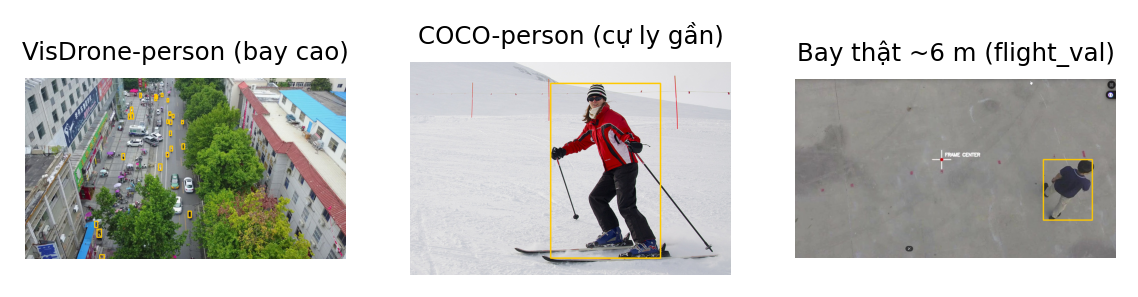
\includegraphics[width=\textwidth]{mau_du_lieu.png}
\caption{Ba nguồn dữ liệu của đề tài và nhãn bounding box tương ứng: VisDrone-person chụp từ trên cao (trái), COCO-person ở cự ly gần (giữa) và khung hình bay thật ở độ cao khoảng 6\,m (phải)}
\label{fig:maudulieu}
\end{figure}

\section{Các bộ dữ liệu}

\subsection{VisDrone-person}

VisDrone2019-DET~\cite{zhu2022visdrone} là bộ dữ liệu phát hiện đối tượng từ UAV do Đại học Thiên Tân (Trung Quốc) công bố, chụp ở nhiều thành phố, độ cao và điều kiện ánh sáng, gồm mười lớp đối tượng. Đề tài chuyển bộ dữ liệu về bài toán một lớp bằng cách gộp hai lớp \texttt{pedestrian} (người đang đi hoặc đứng) và \texttt{people} (người ở tư thế khác như ngồi) thành lớp \textit{person}, vì hệ thống bám theo phải nhận ra người ở mọi tư thế. Các hộp có cạnh nhỏ hơn 10 điểm ảnh bị loại vì gần như không thể gán nhãn nhất quán. Nhãn được chuyển sang định dạng YOLO (tâm, rộng, cao chuẩn hoá về $[0,1]$). Kết quả gồm 6.471 ảnh huấn luyện với 65.523 hộp và 548 ảnh kiểm định với 8.165 hộp. Trong tập kiểm định, 98,7\% số hộp có diện tích dưới $32^2$ điểm ảnh sau khi đưa ảnh về $640\times640$, nên AP trên tập này gần như trùng với AP của vật nhỏ.

\subsection{COCO-person}

COCO~\cite{lin2014coco} chứa ảnh đời thường với người ở cự ly gần và nhiều tư thế. Đề tài lấy các chú thích lớp \textit{person} từ tập val2017, bỏ những hộp có diện tích dưới 100 điểm ảnh vuông, được 2.654 ảnh với 9.783 hộp. Tập này bổ sung cho mô hình kinh nghiệm về người kích thước lớn mà VisDrone gần như không có. Khi dùng, mỗi epoch trộn thêm một lượng ảnh COCO bằng 25\% số ảnh VisDrone (1.618 ảnh).

\subsection{Tập bay thật flight\_val}

Tập này được xây dựng từ chuyến bay thử ngày 21/07/2026 trên một bãi nền bê tông. Máy bay bay ở chế độ giữ vị trí, độ cao khoảng 6\,m, camera nhìn xuống, một người đi bộ bên dưới. Video được ghi từ màn hình trạm mặt đất, vùng giao diện được cắt bỏ, và một khung hình được lấy mỗi giây trong đoạn bay ổn định từ giây thứ 18 tới giây thứ 150. Nhãn được khởi tạo bằng mô hình rồi sửa tay từng khung trên công cụ Roboflow theo bộ quy tắc: hộp ôm sát toàn thân nhìn thấy, xoá mọi hộp sai (bóng, vết bẩn nền, biểu tượng giao diện), bổ sung người bị bỏ sót. Sau khi rà soát còn 92 khung hình $1174\times654$, mỗi khung có đúng một người. Tập này \textit{không} được dùng để huấn luyện, chọn mô hình hay hiệu chuẩn lượng tử hoá; nó chỉ dùng để đánh giá, nhằm tránh rò rỉ dữ liệu.

\begin{table}[H]
\centering
\caption{Thống kê ba bộ dữ liệu sau chuẩn hoá (lớp duy nhất \textit{person})}
\label{tab:dulieu}
\small
\renewcommand{\arraystretch}{1.15}
\begin{tabularx}{\textwidth}{@{}l>{\centering\arraybackslash}X>{\centering\arraybackslash}X>{\centering\arraybackslash}X>{\raggedright\arraybackslash}p{4.2cm}@{}}
\toprule
\textbf{Bộ dữ liệu} & \textbf{Số ảnh} & \textbf{Số hộp} & \textbf{Trung vị diện tích hộp @640 (px$^2$)} & \textbf{Vai trò}\\
\midrule
VisDrone-person huấn luyện & 6.471 & 65.523 & -- & Huấn luyện\\
VisDrone-person kiểm định & 548 & 8.165 & 122 & Chọn mô hình, so sánh, đánh giá rung\\
COCO-person & 2.654 & 9.783 & -- & Bổ sung người cự ly gần (nhánh triển khai)\\
flight\_val (bay thật $\approx$6\,m) & 92 & 92 & 7.874 & Chỉ đánh giá trên miền triển khai\\
\bottomrule
\end{tabularx}
\end{table}

\section{Hai nhánh mô hình}
\label{sec:hainhanh}

Để vừa so sánh công bằng với các công trình khác, vừa phục vụ triển khai thật, đề tài duy trì hai nhánh huấn luyện độc lập dùng chung một kiến trúc:
\begin{itemize}
\item \textbf{Nhánh chuẩn:} chỉ huấn luyện trên VisDrone-person, không thêm dữ liệu ngoài. Mọi bảng so sánh với mô hình đối chứng dùng nhánh này, để chênh lệch không đến từ dữ liệu bổ sung.
\item \textbf{Nhánh triển khai:} huấn luyện trên VisDrone-person trộn COCO-person, nhắm tới người ở cự ly gần. Mô hình chạy trên máy bay thuộc nhánh này.
\end{itemize}

\section{Tiền xử lý và data augmentation}

Ảnh được co giãn giữ nguyên tỷ lệ về cạnh dài 640 điểm ảnh và đệm phần thiếu bằng màu xám (letterbox), toạ độ nhãn được biến đổi tương ứng. Trong huấn luyện, đề tài dùng các phép tăng cường chuẩn: ghép bốn ảnh (xác suất 0,5, tắt ở các epoch cuối để mô hình quen với ảnh đơn), trộn hai ảnh (0,1), lật ngang (0,5), biến đổi affine, thay đổi màu, sao chép dán đối tượng (0,4), một số phép biến đổi đặc thù ảnh UAV (0,3), và huấn luyện đa tỷ lệ với kích thước ảnh ngẫu nhiên từ 50\% tới 100\% của 640, bước 32 điểm ảnh. Các phép này đều là những biến đổi mà dữ liệu gốc đã phần nào chứa đựng; không phép nào mô phỏng rung của khung máy bay. Suy giảm do rung được đưa vào riêng ở Chương~\ref{chap:mohinh}.

\section{Giao thức mô phỏng rung VisDrone-Shake}
\label{sec:shake}

\subsection{Mô hình suy giảm}

Giao thức hiện thực phương trình~(\ref{eq:rung}) trên ảnh đã chuẩn hoá về $[0,1]$ theo ba bước: (1) tích chập theo từng kênh màu với nhân nhoè dạng đoạn thẳng dài $L$ điểm ảnh, hướng $\theta$ lấy ngẫu nhiên đều trong $[0^\circ, 180^\circ)$, nhân được chuẩn hoá tổng bằng 1; (2) cộng nhiễu Gauss độ lệch chuẩn $\sigma$; (3) nhân toàn ảnh với hệ số $1+u$, $u$ lấy đều trong $[-b, b]$. Ba mức suy giảm được định nghĩa trong Bảng~\ref{tab:shake} và minh hoạ ở Hình~\ref{fig:rungminhhoa}. Mức 1 và mức 2 tương ứng máy bay cân bằng tốt đang bay ổn định hoặc bay tiến; mức 3 tương ứng kích thích mạnh như cánh quạt mất cân bằng.

\begin{table}[H]
\centering
\caption{Tham số ba mức rung của giao thức VisDrone-Shake}
\label{tab:shake}
\small
\renewcommand{\arraystretch}{1.15}
\begin{tabular}{@{}lcccl@{}}
\toprule
\textbf{Mức} & \textbf{Độ dài nhoè $L$ (px)} & \textbf{Nhiễu $\sigma$} & \textbf{Dao động sáng $b$} & \textbf{Tình huống tương ứng}\\
\midrule
Mức 1 & 5 & 0,02 & $\pm$10\% & Bay treo, khung cân bằng tốt\\
Mức 2 & 9 & 0,04 & $\pm$20\% & Bay tiến thông thường\\
Mức 3 & 15 & 0,06 & $\pm$30\% & Kích thích mạnh (cánh quạt lệch)\\
\bottomrule
\end{tabular}
\end{table}

\begin{figure}[H]
\centering
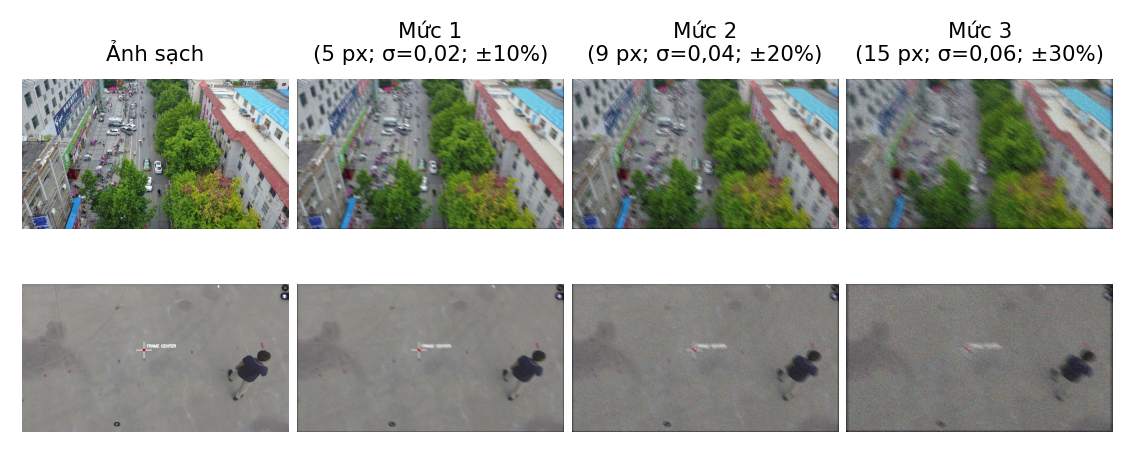
\includegraphics[width=\textwidth]{rung_minh_hoa.png}
\caption{Minh hoạ ba mức rung VisDrone-Shake trên một ảnh VisDrone (hàng trên) và một khung bay thật (hàng dưới); hướng nhoè cố định $35^\circ$ để dễ so sánh}
\label{fig:rungminhhoa}
\end{figure}

Điểm quan trọng là không bước nào trong ba bước làm dịch chuyển đối tượng: nhoè đối xứng quanh tâm, nhiễu và độ sáng không đổi hình học. Vì vậy bounding box gốc vẫn hợp lệ trên ảnh đã suy giảm, và cùng một toán tử có thể dùng cho cả đánh giá lẫn huấn luyện mà không phải sửa nhãn.

\subsection{Giao thức phải được cố định seed ngẫu nhiên}

Hướng nhoè, nhiễu và độ sáng đều được rút ngẫu nhiên, nên một lần chạy đánh giá chỉ là một lần rút thăm. Trong quá trình làm đề tài, nhóm đã đo cùng một checkpoint ba lần mà không cố định hạt giống và nhận được tỷ lệ retain 17,0\%, 17,1\% và 17,6\%, tức dao động hơn nửa điểm phần trăm, đủ để tạo ra một ``cải tiến'' giả. Giao thức chính thức vì thế gieo lại hạt giống trước \textit{mỗi} lượt đánh giá ở mỗi mức, chạy với ba hạt giống 0, 1, 2 và báo cáo trung bình $\pm$ độ lệch chuẩn mẫu. Đánh giá trên ảnh sạch là tất định nên chỉ chạy một lần. Chỉ số tổng hợp là mCP và retain theo phương trình~(\ref{eq:mcp}) với $M=3$.

\section{Một chương trình đo duy nhất cho mọi mô hình}
\label{sec:mottrinhdo}

Mỗi họ mô hình đi kèm chương trình đánh giá riêng với ngưỡng tin cậy, số hộp tối đa và quy ước diện tích khác nhau. Khi đo lại YOLOv8-n bằng chương trình của Ultralytics, nhóm được AP@[.50:.95] = 0,2787; khi đo bằng chương trình chung của đề tài, được 0,2684. Chênh lệch 0,01 này cùng cỡ với khoảng cách giữa các mô hình đối chứng với nhau, nên nếu trộn hai chương trình đo trong cùng một bảng, người đọc sẽ nhầm khác biệt do cách đo thành khác biệt giữa các mô hình. Với RT-DETR-l chênh lệch còn lớn hơn (0,3340 so với 0,2502), vì bộ tiền xử lý gốc của nó kéo giãn ảnh cho vuông thay vì đệm xám.

Do đó, \textbf{mọi mô hình trong mọi bảng của Chương~\ref{chap:ketqua}} được đo bằng một chương trình duy nhất (\texttt{paper\_eval\_unified.py}) với cùng cấu hình:
\begin{itemize}
\item cùng bộ nạp ảnh letterbox $640\times640$, mọi mô hình nhận đúng cùng một tensor đầu vào;
\item ngưỡng tin cậy 0,01, NMS với ngưỡng IoU 0,5, tối đa 300 hộp mỗi ảnh;
\item chấm điểm bằng thư viện \texttt{pycocotools} trên cùng một tệp nhãn chuẩn;
\item ba hạt giống cho mọi lượt đánh giá có rung.
\end{itemize}
Chỉ số retain không bị ảnh hưởng bởi cách tiền xử lý của từng mô hình vì nó là tỷ số giữa hai lượt đo trong cùng một đường xử lý; tuy vậy, đề tài vẫn ghi chú rõ trường hợp RT-DETR-l trong bảng kết quả.

\section{Quy tắc chọn checkpoint}

Mỗi lần huấn luyện sinh ra checkpoint tốt nhất theo AP kiểm định trên ảnh sạch (\texttt{best.pt}) và checkpoint cuối (\texttt{last.pt}). Với SteadyDet-W được huấn luyện có ràng buộc nhất quán, \texttt{last.pt} cho retain 33,4\% còn \texttt{best.pt} cho 30,5\%. Nếu lấy \texttt{last.pt} cho mô hình của mình và \texttt{best.pt} cho mô hình đối chứng thì đó là hai quy tắc khác nhau và kết quả bị thiên vị. Đề tài áp dụng một quy tắc duy nhất: \textbf{mọi mô hình dùng checkpoint tốt nhất theo AP sạch}, không checkpoint nào được chọn dựa trên chính giao thức rung dùng để đánh giá nó.

\section{Đánh giá trên miền triển khai}

Trên tập flight\_val, các mô hình được đánh giá bằng hai cách bổ trợ. Cách thứ nhất dùng cùng hàm \texttt{pycocotools} để tính AP@0,5, AP@[.50:.95], AP@0,75 và AR@100. Vì chỉ có 92 khung, đề tài lấy mẫu lại khung hình 1.000 lần theo phương pháp bootstrap ghép cặp để tính khoảng tin cậy 95\% cho hiệu giữa hai mô hình. Cách thứ hai sát với vận hành hơn: chạy mô hình một lần ở ngưỡng tin cậy thấp 0,02 rồi quét ngưỡng ngoại tuyến, tại mỗi ngưỡng ghép dự đoán với nhãn bằng IoU $\ge 0{,}5$ để tính precision, recall, F1 và số hộp sai mỗi khung. Ngưỡng cho F1 cao nhất được chọn làm ngưỡng vận hành trên máy bay.

Khi so sánh mô hình FP32 và INT8, cả hai được xuất dự đoán ra cùng một định dạng và chấm bằng cùng một hàm, để chênh lệch chỉ phản ánh tác động của lượng tử hoá.

\section{Môi trường thực nghiệm}

\begin{table}[H]
\centering
\caption{Môi trường phần cứng và phần mềm dùng trong đề tài}
\label{tab:moitruong}
\small
\renewcommand{\arraystretch}{1.15}
\begin{tabularx}{\textwidth}{@{}l>{\raggedright\arraybackslash}X@{}}
\toprule
\textbf{Hạng mục} & \textbf{Cấu hình}\\
\midrule
Máy huấn luyện & Máy tính xách tay GPU NVIDIA RTX 4060 Laptop 8\,GB, RAM 14\,GB, CUDA; PyTorch; Ultralytics 8.4 cho các mô hình đối chứng\\
Máy tính trên UAV & Raspberry Pi~5 (Debian 12, nhân 6.12, aarch64), Python 3.11\\
Bộ tăng tốc & Hailo-8L qua PCIe, HailoRT 4.20.0; biên dịch bằng Hailo Dataflow Compiler 3.34 trên máy x86\\
Camera & Logitech C270 HD, USB, MJPG, tối đa $1280\times720$ ở 30 khung hình/giây\\
Bộ điều khiển bay & Holybro Pixhawk~6C, ArduPilot Copter 4.7.0, kết nối USB, MAVLink v2\\
Phần mềm hỗ trợ & Mission Planner (cấu hình tham số), pymavlink, OpenCV, NumPy, SciPy\\
\bottomrule
\end{tabularx}
\end{table}

\section{Kết luận chương}

Đề tài sử dụng ba nguồn dữ liệu bao phủ hai miền: VisDrone-person cho so sánh chuẩn, COCO-person bổ sung người cự ly gần, và 92 khung bay thật chỉ dùng để đánh giá trên miền triển khai. Giao thức VisDrone-Shake mô phỏng ba hiệu ứng vật lý của rung mà không làm sai nhãn, được cố định seed và lặp ba lần. Mọi mô hình được đo bằng một chương trình duy nhất và chọn checkpoint theo một quy tắc duy nhất. Những ràng buộc này đảm bảo các so sánh ở Chương~\ref{chap:ketqua} phản ánh khác biệt thật giữa các mô hình.
